\documentclass{article}
\usepackage{times}
\usepackage{geometry}
\usepackage{multicol}
\usepackage{graphicx}
\usepackage{comment}
\usepackage{float}
\usepackage[%  
    colorlinks=true,
    citecolor=cyan,
    pdfborder={0 0 0},
    linkcolor=red
]{hyperref}




\geometry{letterpaper, textwidth=6.5in, textheight=9in}

\title{Dining Hall Occupancy Estimation using Computer Vision}
\author{
  Riju Dey\\
  rd3054\\
  Columbia University\\
  rd3054@columbia.edu
  \and
  Nick Martin\\
  njm2175\\
  Columbia University\\
  njm2175@columbia.edu
}

\begin{document}


\maketitle

\section*{Abstract}
  The current system to track how full a dining hall is on campus is woefully inadequate. A tracker is available for each dining hall on the Columbia Dining website, yet these measures are often inaccurate or entirely implausible (for instance, a capacity of 300\% full). This occupancy measurement is based upon the number of wifi signals that it detects within the dining hall, which is subject to many issues, including stray connections within the building that should not be counted, and simply inaccurate counting of active wifi connections. We present a dataset of ~3000 unique dining hall images and several models that achieve over ~70\% accuracy on unseen data after training.

GitHub repo: https://github.com/UjirYed/AppliedComputerVision


\begin{multicols}{2}
\section{Introduction}
\subsection*{Problem Statement}
The Columbia Dining website features a seating capacity indicator for each of their dining halls. Ostensibly a helpful way for students to avoid overcrowding in dining halls, the authors of this paper-as Columbia undergraduates-can attest to the fact that it is often unreliable. It isn't rare for there to be a significant mismatch between the online indicator and real life-and sometimes the indicator even breaks entirely (Fig \ref{fig:fig1})!


\begin{figure}[H]
  \centering
  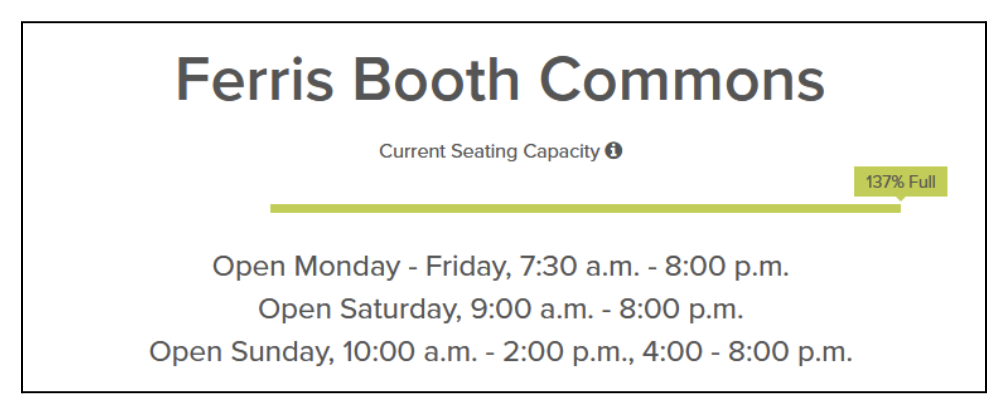
\includegraphics[width=0.4\textwidth]{fig1.png}
  \caption{Ferris Booth Commons is 137\% full.}
  \label{fig:fig1}
\end{figure}

%\columnbreak

Run by Occuspace, these indicators use “detect WiFi and Bluetooth signals from electronic devices” to make an estimate about how many people are in the room. Clearly, however, this is far from a perfect system.

On the other hand, we also sought inspiration from a far more functional website-Google's "Popular Times" feature, depicts how "busy" a certain area (e.g. a restaurant, or a mall) is by classifying it as "busy," "not busy," or a similar category over several periods of time. For instance, in Fig. \ref{fig:fig2}, we see how “Popular Times” gives a qualitative measurement of a restaurant's busyness, saying it's “not too busy” and plotting its estimate on a rough bar graph.

\begin{figure}[H]
  \centering
  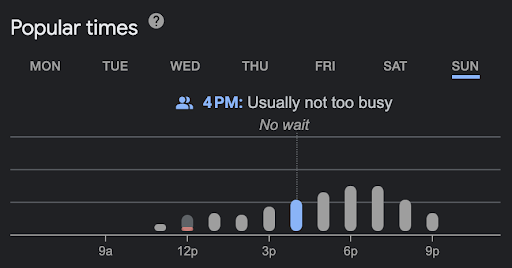
\includegraphics[width=0.4\textwidth]{fig2.png}
  \caption{Google's Popular Times graph shows the distribution of busyness over time.}
  \label{fig:fig2}
\end{figure}


\subsection*{Objective}
The goal of our project is to develop a meme classification framework that can accurately interpret and categorize hateful memes. We want to use the Visual Language Model (VLM)'s powerful ability of interpreting both visual and textual data to help us understand meme. This project aims to improve current categorization methods, and to address the hateful meme classification challenge. The final goal of the project is to help people to better regulate content, thereby protecting users from offensive content, and to promote the development of ethical and responsible AI technologies that contribute to a safer online environment.

Unfortunately, these assessments are only made possible through Google’s unique position to enact large-scale surveillance on its network of users; for instance, through tracking the location of Android phones and Google Maps users. This presents an issue for other entities such as universities, which may want to implement a similar system but cannot use the same means–people may feel uncomfortable having their location information collected, and it’s pretty unfeasible for most companies other than Google to obtain so much of this data.

Working off these two ideas, we came up with a potential solution to Columbia’s dining hall problem which could be easily implemented and maintain a respectable level of user privacy like the current system, while also giving an accurate and useful categorization like the Google feature does. By using a computer vision system to determine how “full” the dining hall looks, we believed we could accurately categorize its capacity into 1 of 5 categories: “not busy,” “a little busy,” “moderately busy,” “busy,” and “extremely busy.” This would then be supplemented with a visual estimate similar to the bar that the Columbia Dining page already presents. Since dining halls already have security cameras, we believe that using visual data to determine dining hall capacity would not present a significant privacy violation. Additionally, though looking at how similar features like “Popular Times” work, we concluded that a rougher estimate on a 1 to 5 scale, in contrast to the current percentage-based system, would be precise enough to be valuable to dining-hall goers. Thus, we set out to create a revised capacity indicator by training a model to visually predict a dining hall’s capacity at any given time.


\section{Related Works}
Measuring "busyness" or "fullness" of a scene is not a new problem. Predicting busyness by itself, however, is often a hard to define notion, so most work has been done on the inverse problem: classifying and detecting free space in a scene. For instance, consider a previous paper on classifying the occupancy of parking lots \cite{marekImageBasedParkingSpace2021}. The researchers of this study used a combination of object detectors and classification models to identify parking individual parking spaces in an image, and then determine whether they are empty. This paper also represents a jump in the quality of data available for such a problem; the researchers stress the importance of having images from unique parking lots and views of each space.

There has also been similar work in the retail space, where models attempt to find voids in shelves to find where items need to be restocked (link). Once again, this project necessitated a custom dataset, and used object detection to find individual empty spaces within an image.

\section{Method Overview}
\subsection*{Data}
Data collection was an extremely difficult part of this project, and definitely the most time-consuming and intensive. We attempted several different procedures of obtaining training data, ultimately creating multiple iterations of our own custom dataset to tackle the problem.

\subsubsection*{Openly Available Image Datasets}
We began our search by attempting to adapt popular datasets to suit our problem. However, most of the traditional large, open-source datasets (COCO, ImageNet) had little to no pictures of dining halls, and were thus not a good fit for our problem \cite{linMicrosoftCOCOCommon2015,russakovskyImageNetLargeScale2015}. Additionally, we found several image datasets of parking lot data (e.g., from the parking space capacity paper), but while they share a similar concept of “fullness,” we didn’t think they would translate very well to our dining hall problem at all.

\begin{figure}[H]
  \centering
  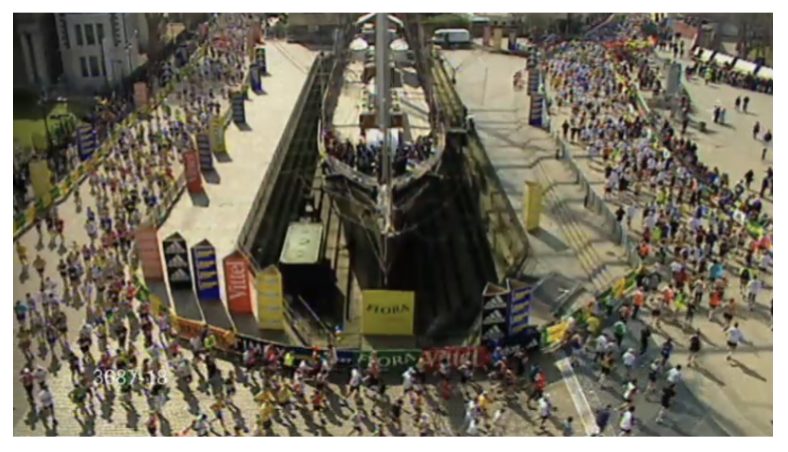
\includegraphics[width=0.4\textwidth]{ucfcrowds.png}
  \caption{A sample image extracted from UCF’s Crowds Dataset.}
  \label{fig:fig4}
\end{figure}

We also looked through several datasets depicting crowds and various human actions. For instance, the CUHK crowd and mall datasets both have a variety of videos showing various levels of crowd density. But while at first sight these seemed to tackle a similar problem to ours, we decided that they would likely not generalize well to dining halls, at least on their own. We also looked at crowd datasets from UCF, but this data tended to show crowds of far greater density than would ever (hopefully) be seen in a dining hall.

\subsubsection*{Manual Collection and Labeling}
Publicly available datasets did not seem to be available to suit our task, so we began to create our own dataset from scratch. We took several photos of dining halls around Columbia, and classified them ourselves based on our judgment of the scene. We also searched Google Images manually and selected high quality images that were representative of each category. To further expand our dataset, we took screenshots from several openly available datasets and online movie clips and videos, which depicted scenes of enclosed rooms with various amounts of people. In the end, we were able to put together a dataset of 88 high quality images.

Although this method is most certainly the "best" way in terms of ensuring data quality, it was time-consuming and difficult to obtain images. Furthermore, using this small dataset to finetune the models we use in this paper (ViT, ResNet) yielded very poor results.

\subsubsection*{Generating Synthetic Data Using Diffusion Models}

\begin{figure}[H]
  \centering
  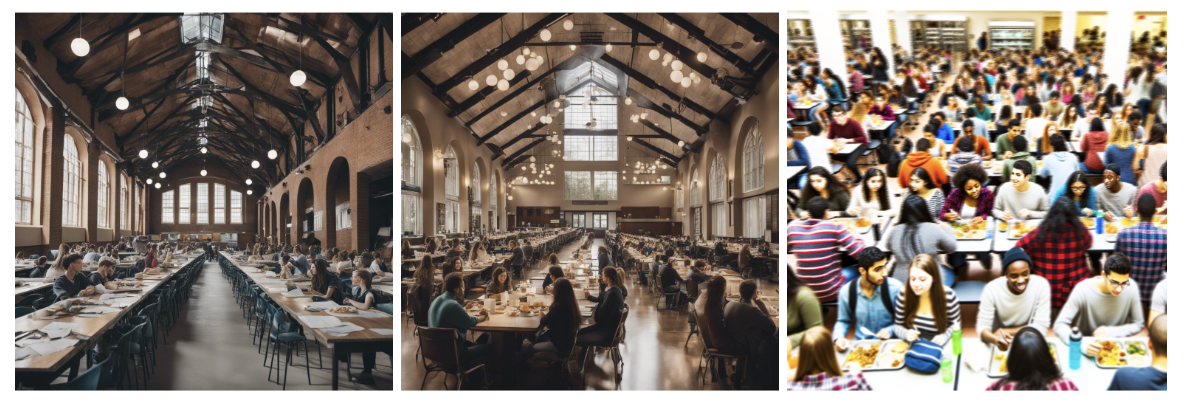
\includegraphics[width=0.45\textwidth]{diffusionImages.png}
  \caption{Diffusion models generated images which lacked variety and weren’t clear.}
  \label{fig:fig3}
\end{figure}

In this case, we prompted a pre-trained diffusion model to generate images of dining halls in various states of occupancy \cite{rombachHighResolutionImageSynthesis2022}. This was done on closed models such as DALL-E and Stable Diffusion as well as open-source models found on Huggingface. In theory, not only would this give us a scalable way to generate high-quality data, it would also give us our labels for free, as they were integrated into the prompt. In practice, however, this does not pan out.

While seemingly a good idea, the diffusion models provided bland and undiverse photos, regardless of how much we varied the prompts for each photo. Tweaking the temperature, style and prompts either did very little to modify the generated photos, or created images that were completely unusable. Furthermore, the generated images were low quality and often blurry, often making it difficult even for us to judge how full they were. Examples of such images are shown in Fig. \ref{fig:fig4}. We concluded these would be unfit for our task and not generalize well to real-life dining halls, so we ultimately left these images out of our dataset.

\subsubsection*{Scraping Google Images Directly}
The method that worked best–and what we ultimately used as the basis for collecting data–was simply manually scraping Google Images. To do so, we adapted code from BrowserPilot (link), which provides a template for a LLM agent that performs web scraping using Selenium. After experimenting with prompts, we were able to generate a script that allowed our GPT-3.5-based Agent to search for and download images from Google, using a variety of prompts which we specified.

We found that although it was functional, the Agent was finicky. The Agent was prone to occasional crashes even when given the same prompt repeatedly, and in the end it may have been faster to simply write the Selenium script ourselves. Nonetheless, it was a valuable experience and we'd postulate that there would be benefits to using an Agent for more abstract queries (especially if we’d expanded our data collection to include web sources beyond Google Images).

After scraping our images, we performed slight data cleaning (i.e., removing duplicates, corrupted images, invalid links). After looping through several different search queries and using the Agent on each, we were able to massively expand our dataset to include 3014 unique images.

\subsubsection*{Labeling the Data}
Now that we had our data, we had to figure out a way to label it on our scale of 1-5. However, labeling over 3000 images by hand would have required a copious amount of manual labor–especially between just two people. So instead, we took cues from model distillation, where, broadly speaking, a larger, more complex "teacher model" is used to train a simpler but less cumbersome "student model.”

To this end, we looked for large pretrained models that generated text from image and text input. We played around with using open-source models such as LLaVa \cite{liuVisualInstructionTuning2023}, but found that the best performance came from the Claude models provided by Anthropic. We then wrote a script and carefully engineered a prompt to coax Claude into generating the most accurate label for each image. We also asked Claude to remove images that were clearly not dining halls, thus doing some of the filtering for us.

After running the script, we found that labels were generally accurate for the lower and higher extremes (sparse/empty and extremely busy), but required some manual modifications for the more subtle categories. Additionally, we built on Claude’s data cleaning by doing some manual sorting to remove clearly incorrectly labeled images and additional images that simply did not depict dining halls.

\begin{figure}[H]
  \centering
  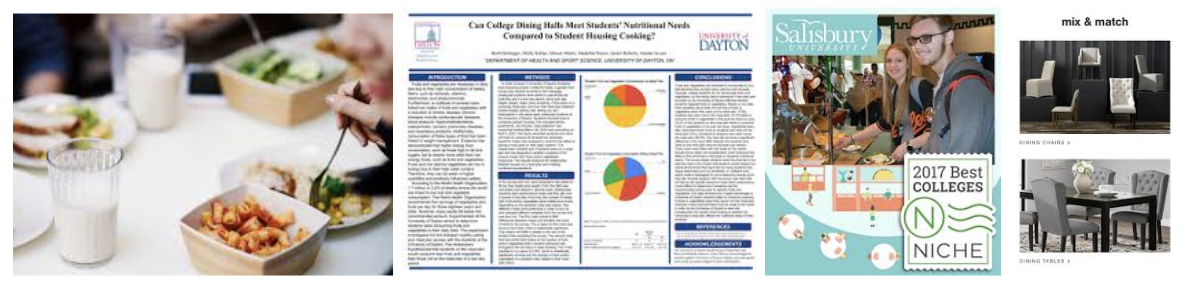
\includegraphics[width=0.45\textwidth]{badScrapedImages.png}
  \caption{The Agent collected various unrelated images which had to be filtered out in labeling.}
  \label{fig:fig3}
\end{figure}

\subsection*{Our Models}

\subsubsection*{ResNet}

Because our problem was a classification task, we naturally turned to the ResNet models. A classic model that saw significant success on classifying ImageNet, it has been a popular choice as a backbone for many future models \cite{elharroussBackbonesReviewFeatureExtraction2022,heDeepResidualLearning2015}.  We attempted to adapt the model to classify images of dining halls. We did this in two different ways: first, we tried to fine-tune a pretrained, ResNet-50. We did this through linear probing–we edited the classifier layer to go from its original 1000 classes to 5, and then froze the entire model except for the classifier head. This both preserved efficiency in our training and allowed us to fine-tune the model slightly for our problem without losing too much of the original training.

Secondly, we also experimented with a custom ResNet, instantiated from scratch. Here, we provided our own embedding, layer sizes, and depths, and started them with entirely random weights. Therefore, for this version, we had to train the entire model, not just the classifier.

\subsubsection*{EfficientNet}
We also experimented with fine-tuning an EfficientNet model–a much smaller and more efficient classification model than ResNet \cite{tanEfficientNetRethinkingModel2020}. Similar to our pretrained ResNet, we used a pretrained EfficientNet-b0 combined with a linear probing technique to fine-tune only the weights of the classifier head.

Due to time, computational constraints and poor initial results, we did not train an EfficientNet from scratch like with the ResNet model.

\subsubsection*{Transformers: ViT and Swin}
In addition to convolutional networks, we also wanted to look at the performance of transformers on this task. Though more computationally intensive to train than the prior two models, we thought that the additional power of transformers might improve accuracy on this task. We first tested a Vision Transformer, or ViT, pretrained on ImageNet, adding a classifier head to correspond to our 5 classes \cite{dosovitskiyImageWorth16x162021}. To improve training efficiency, we also took advantage of LoRA (as described below) when fine-tuning this model.
Similarly to the ViT, we took a Swin V2 transformer \cite{liuSwinTransformerV22022} pretrained on ImageNet, and added our own classifier head. For this transformer we also used LoRA to optimize training efficiency.

\subsubsection*{Concatenation Model (ResNet + YOLO)}
We also tested a concatenation model to further improve our results, combining the benefits of a classifier (ResNet) and object detector (YOLO). This model takes the hidden states of the YOLO transformer and the ResNet, concatenates them, and then passes them through a classifier layer. We finetuned a pretrained YOLO model with LoRA, and we tested with ResNets pretrained on ImageNet as well as those fine-tuned to our dataset.

\section*{Experiments and Analysis}

\subsection*{Training}
For each model described in the previous section, we trained them with Hugging Face’s trainer module, manipulating several variables. We tested base learning rates of 1e-3 and 3e-4, batch sizes 64 and 128, and varied dropout between 0 and 0.2. For each of these combinations, we trained for 100 epochs, saving both the best epoch as well as the final one for reference. Once all models were finished training, we compared performance between models and selected the best performing one overall. The learning rates and batch sizes were chosen after preliminary testing. Using batch sizes lower than 64, or learning rates lower than 1e-3, would cause NaN/Inf losses. The default Cross-Entropy loss function was used for all models. We played around with weighting classes differently, but found it had minimal impact.

\subsection*{Evaluation}

Since our problem was a straightforward classification task, we elected to use validation set accuracy as our evaluation strategy. Our dataset of 3014 images was split into a training set of 2981 and a validation set of 33 (containing at least 5 images of each class). At the end of each epoch, we calculated the percentage of the validation set our model correctly predicted, saving the best epochs accordingly. To avoid overfitting, the model that achieved the best validation accuracy earliest was saved. Training and saving the models was done automatically via Hugging Face’s Trainer for all of our models.

\begin{figure}[H]
  \centering
  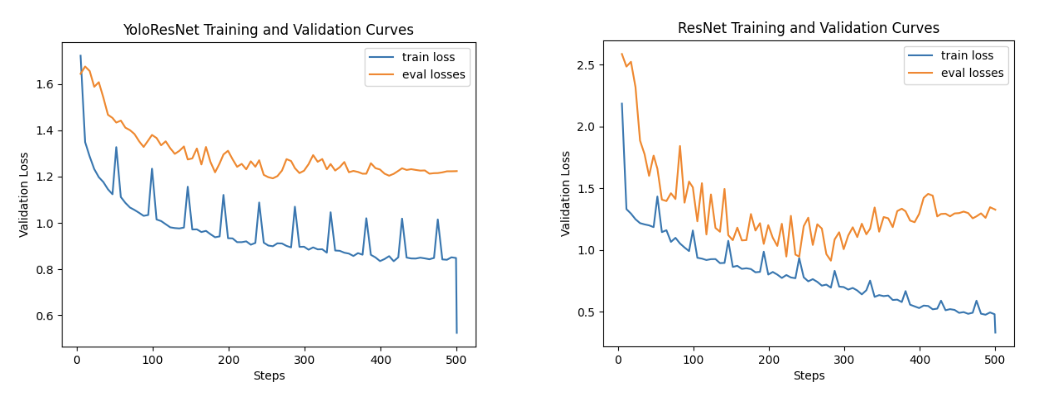
\includegraphics[width=0.49\textwidth]{trainingcurves.png}
  \caption{Selected training and validation loss curves from training. Due to the small batch (smaller than the specified batchsize) that occurs at the very end of each epoch, a regular spike in training loss is observed every 50 steps.}
  \label{fig:fig6}
\end{figure}

\subsection*{Analysis of Results}


Using our best model, we also computed a confusion matrix of the model's performance on the training dataset, to see where it struggled and find potential areas of improvement. We observed that classes of 1, 3, and 4 (sparse, moderately busy, and very busy) were classified reasonably well, with almost all predictions being within one class of the ground truth. For class 2 (somewhat busy), we found that the model had trouble predicting the correct label, but was often within 1 of the correct answer. 

\begin{figure}[H]
  \centering
  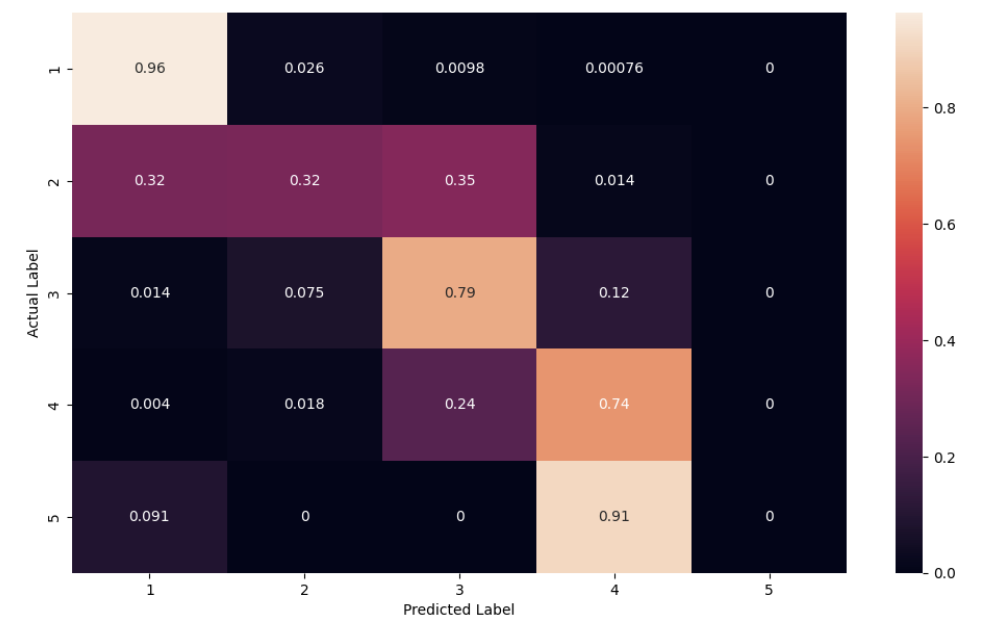
\includegraphics[width=0.45\textwidth]{confusionMatrix.png}
  \caption{A confusion matrix of our best-performing concatenation model.}
  \label{fig:fig7}
\end{figure}


We would attribute this to the fact that the notion of "somewhat busy" is already somewhat vague, and thus hard to always predict accurately. Therefore, our auto labeling procedure may not have been very consistent, leading to inconsistently labeled data in this category. 
  
Furthermore, our model simply does not label any images as class 5, or "extremely busy". This is likely due to the fact that we only had ~20 training images for this class, compared to hundreds for the other classes. This was one of the most difficult challenges we encountered during this project, and were unfortunately unable to fix–even after performing various experiments, such as reweighting losses.

\end{multicols}
\begin{table} [H]
  \renewcommand{\arraystretch}{1.2}
  \caption{Model Performance}
  \label{table_example}
  \centering
  \begin{tabular}{|c|c|c|c|c|}
    \hline
  Model & Batch Size & Base LR & Dropout & Accuracy\\
  \hline
  ResNet (scratch) & 128 & 3e-4 & 0 & 69.7 \\
  \hline
  ResNet (pretrained) & 128 & 1e-3 & 0.2 & 54.5 \\
  \hline
  EfficientNet (pretrained) & 64 & 1e-3 & 0.2 & 63.6 \\
  \hline
  ViT (pretrained) & 64 & 1e-3 & 0 & 69.7 \\
  \hline
  SwinV2 (pretrained) & 64 & 3e-4 & 0.2 & 69.7 \\
  \hline
  \textbf{Concat (YOLO + ResNet)} & 64 & 3e-4 & 0 & \textbf{72.7} \\
  \hline
  \end{tabular}
\end{table}

\begin{multicols}{2}
\section*{Web Application}
Now that we had our model, we created a web interface to test our project in a similar way to real-life. We created a website that allows the user to upload a photo of a dining hall, which is then classified into a busyness category by our model. The website then displays text and a bar showing how full the dining hall is. See Fig. \ref{fig:fig8} for a simple demonstration of this web app.

A real world implementation of this model would function in much the same way. Our model can be uploaded onboard a small computer or camera, which occasionally takes pictures of a dining hall. The picture is then passed through the model, obtaining a classification, which can be pushed to the dining hall’s website. 

\section*{Conclusions}

\subsection*{Findings}
Ultimately, our models showed a fair amount of success in autonomously classifying the capacity of dining halls. Through the creation of a custom dataset, scraped from Google Images, we were able to gather enough data to train our model with a good degree of accuracy. Additionally, our model is extremely transferable to real-world use–unlike large LLMs like Claude or GPT, our models are lightweight enough to fit on a camera or small computer, without losing too much accuracy in comparison to the larger models.
\begin{figure}[H]
  \centering
  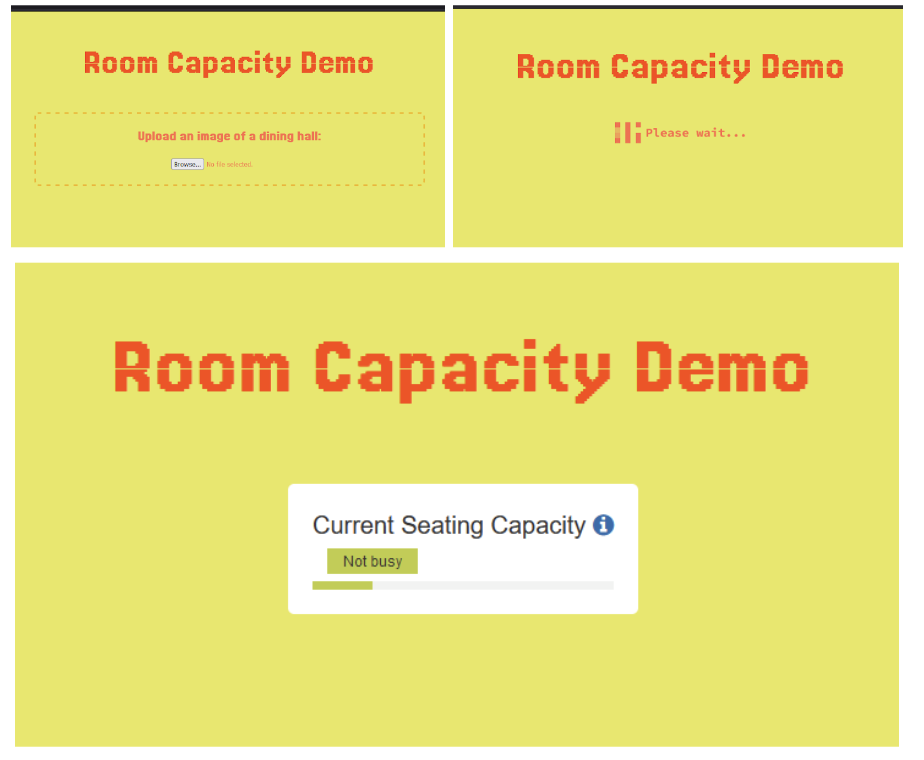
\includegraphics[width=0.45\textwidth]{webapp.png}
  \caption{Demonstration of dining hall web app. The user uploads an image of a dining hall, which is then processed and classified.}
  \label{fig:fig8}
\end{figure}
While further training and experimentation would certainly result in even higher accuracy, even our current models seem to be far more accurate than Columbia Dining’s current system on their website. As such, we propose that a computer vision-based system would present a marked improvement upon the current method of tracking WiFi and Bluetooth signals, without being a significant intrusion on privacy. And even though our models solve this via classification, which is less granular than Occuspace’s percentages, we believe classification is a perfectly adequate amount of information for students–going beyond this would simply make our models less efficient for the sake of very limited returns.

\subsection*{Limitations}
As with any machine learning problem, much of the model quality ultimately depends on the data used to train it. While we did end up getting a few thousand images, and effectively sorted out some of the noise, there likely was still a decent amount of incorrect data within our dataset. Additionally, simply collecting data from online sources might not be the best place to get pictures of dining halls specifically, as a lot of our data overlapped with similar things like restaurants or dining rooms. Furthermore, our dataset was imbalanced, especially with respect to class 5, which led to our model being unable to accurately classify such scenes.

Similarly, we were likely limited by our labeling system. Since we used Claude, another model, to create the labels for our data, we are essentially restricting our results to be only as accurate as Claude is. In other words, even if we reached 100\% accuracy on our dataset, our model would still be subject to making mistakes if Claude did as well. In our own testing, we found that while Claude was accurate enough for our purposes, it was far from perfect–thus, our models couldn’t be perfect either.

Finally, we were limited by the model architectures that we had the time and computational capacity to train. For this project, we tested both convolution-based classifiers and transformers, as well as a concatenation model; however, it is possible that other, more advanced models may tackle the problem better while maintaining our desired level of efficiency.

\subsection*{Future Work}
In the future, we believe that taking the time to create an entirely original dataset of new dining hall pictures may allow for some improvement. For instance, by setting up cameras at varying angles in a variety of college dining halls, and then taking pictures throughout the day, one could feasibly construct a much cleaner dataset than the one we scraped from Google. With access to a sufficient variety of dining halls, it would definitely be possible to harvest thousands of new images in just a few weeks. This could even be supplemented by online images for additional variety!

To improve the labeling system, we would suggest moving beyond an LLM-based labeling system, and attempt to label the data by hand. While we did not have the bandwidth for manual labeling in this project, future iterations could pay volunteers to sort the data into categories–which would likely be more reliable and accurate than Claude. Additionally, our 1-5 categories might be too vague and difficult for both humans and LLMs to delineate between–in the future, fleshing these categories out with more description may be helpful. 

Experimenting with different model architectures would also likely yield better results. From our results, it seems that a sole ResNet or ViT might not be the most effective model–the concatenation model, which incorporated an object detector, outperformed the singular models. In response, we propose a more advanced hybrid model for future testing; perhaps one resembling an early fusion model rather than a simple concatenation model. For instance, embeddings from Meta’s SAM \cite{kirillovSegmentAnything2023}, or an object detector, could be passed through a modified ResNet or other classification model. This method may preserve more of the information from the object detector, allowing the ResNet to classify each person or chair in the scene and gain a better understanding of how “full” it really is.

We would also be interested in exploring a larger class of fine-tuning methods. Prefix tuning, which attaches a small learnable vector to the beginning of the input token sequence to better fit to the classification task. Specifically, It would be interesting to apply this to the large open-source transformer models we use for auto labeling to generate more accurate labels. Similarly, adapter-based finetuning, where extra trainable parameters are added to each layer of the existing network to learn task-specific information (in our case, dining-hall specific features) might improve the ability of the network to retain relevant information over time.

In the future, this work may also be expanded to more general scenes, not only those of dining halls.

\section*{Individual Contributions}
Both team members contributed across all parts of the project. Nick was primarily responsible for creating the webapp and writing the train script, as well as helping with cleaning the data before and after labeling. Riju primarily worked on data collection, writing the LLM Agent to both collect and label the data automatically. He also contributed to the train script and evaluation of the trained models. Many of the models themselves were written collaboratively, and code reviews were conducted in person with each member reading through the other’s code.

\end{multicols}

\newpage
\bibliographystyle{alpha}
\bibliography{references}

\end{document}